\section{光的特性}
\subsection{光}
<<<<<<< Updated upstream
\subsection{光学}
=======
\begin{frame}
    \frametitle{光}
    光是眼睛所能看见的电磁辐射。电磁辐射可以被描述为能量波。与其他波一样,电磁波具有\bf{波长}(相邻波峰或波谷的间距);\bf{频率}(每秒波的个数);\bf{幅度}(波峰波谷的差距)。
    \begin{figure}
        \centering
        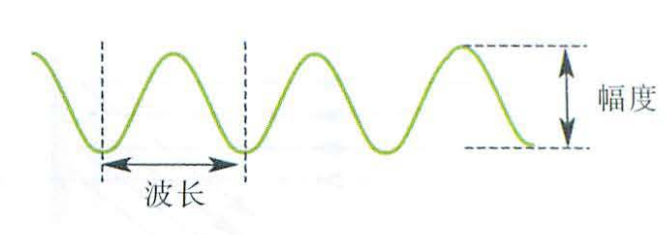
\includegraphics{img/sec1-1.png}
        \caption{电磁波的特点\label{sec1-1}}
    \end{figure}
    \begin{figure}
        \centering
        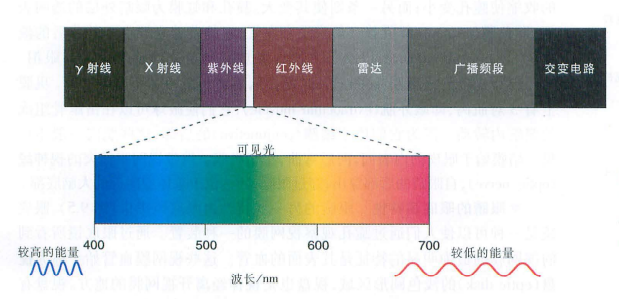
\includegraphics{img/sec1-2.png}
        \caption{电磁频谱\label{sec1-2}}
    \end{figure}
\end{frame}
    电磁辐射的能量的容纳是和它的频率成正比,与波长呈反比。
\subsection{光学}
\begin{frame}
    \frametitle{光学}

    \begin{columns}
            \column{.6\textwidth}{
            在真空中,电磁辐射波沿直线传播。在大气中光也可近似为直线传播,
            直到光与物体表面的原子或者分子发生交互作用。这些相互作用包括反射、吸收和折射。
            \begin{itemize}
                \item 反射是光线在物体表面的反弹。例如镜子的反光。
                \item 吸收是光能在粒子或者表面的转换。例如光能转换为热能。
                \item 折射是光通过介质分界面的弯折。眼睛中的图像通过光的\bf{折射}到达视网膜。
            \end{itemize}
        }
        \column{.4\textwidth}{
            \begin{figure}
                \centering
                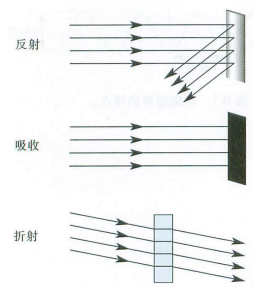
\includegraphics{img/sec1-3.png}
                \caption{光与环境的相互作用\label{sec1-3}}
            \end{figure}
        }
    \end{columns}

\end{frame}
>>>>>>> Stashed changes
